%
\documentclass[Proceedings]{ascelike}
%
% Feb. 14, 2013
%
% Some useful packages...
%
\usepackage{graphicx}
%\usepackage{subfigure}
\usepackage{amsmath}
%\usepackage{amsfonts}
%\usepackage{amssymb}
%\usepackage{amsbsy}
%\usepackage{times}
%
%
% Place hyperlinks within the pdf file (works only with pdflatex, not latex)
% \usepackage[colorlinks=true,citecolor=red,linkcolor=black]{hyperref}
%
%
% NOTE: Don't include the \NameTag{<your name>} if you have selected 
%       the NoPageNumbers option: this leads to an inconsistency and
%       a warning, and the NameTag is ignored.
%\NameTag{Kuhn, Feb. 14, 2013}
%
%
\begin{document}
%
% You will need to make the title all-caps
\title{Determinaci\'on del periodo de la orbita de una estrella binaria espectrosc\'opica.}
%
\author{
Nicolas Garavito-Camargo,%
%
% ---- The first of two styles for addresses: using footnotes and \thanks ----
\thanks{
Dept.\ de F\'isica.,
Universidad de los Andes, 
Cra 1 Nº 18A- 12\ Bogot\'a, Colombia. E-mail: jn.garavito57@uniandes.edu.co}
\ Benjamin Oostra\footnotemark[1]
%
% Adding a second author with the same affiliation (still using \thanks):
%  \\
 %Colleague,\footnotemark[1] Member, ASCE%
%
% Adding another author with a different affiliation.  I have found that 
% the \and command doesn't quite work, so just use "and", as in the following 
% \\
% and
% Younyee Kuhn%
% \thanks{Flourishing wife of same.},%
% \ Not a Member, ASCE
%
% ---- The second of two styles for addresses: below names, no footnotes ----
%
% For this style, don't use \thanks.  Instead, use superscripts and carriage
% returns ("\\").  It's not pretty, but neither is the new ASCE proceedings
% style.  Something like the following:
%
% Matthew R. Kuhn$^1$, Member, ASCE\\[1ex]%
%
% $^1$\parbox[t]{5.75in}{Dept.\ of Civil Engrg.,
% Donald P.\ Shiley School of Engrg., Univ.\ of Portland, 
% 5000 N.\ Willamette Blvd., Portland, OR  97203. kuhn@up.edu.}
}
%
\maketitle
%

\section*{Introducci\'on}

En astronom\'ia a diferencia de la f\'isica no se pueden realizar experimentos ya
que solo hay un universo observable. Por lo tanto de este se tiene que obtener 
toda la informaci\'on posible por medio de observaciones y con estas poder entender 
los fen\'onemos f\'isicos presentes en el universo.

A partir de estas observaciones en particular de la espectroscop\'ia se obtiene informaci\'on,
sobre la abundancia de elementos quimicos, las velocidades radiales, tasas de formacion estelar, 
masas de estrellas etc.

Estas observaciones son de la radiaci\'on proveniente del universo y se hacen
 en diferentes longitudes de onda del espectro electromagnetico. Estas longitudes 
 de onda se dividen en: Microondas, Rayos X, Infrarojo, Visible, Radio, UV. La observaci\'on 
 en estas frecuencias depende en gran medida de las ventanas presentes en la atmosfera terrestre.
Las principales ventanas se encuentran en el rango visible y en ondas de radio por lo que muchos telescopios terrestres son de este tipo. 

El objetivo de este trabajo es familiarizarse con las tecnicas observacionales en astronomia en particular
con el uso de espectros astron\'omicos, para esto se pretende observar una estrella binaria $\varepsilon$ CRA 
y encontrar su periodo orbital a partir de la medici\'on de su espectro. Este estudio por medio de espectros es muy utilizado en astronomia y estudiar estrellas binarias es de gran importancia ya que se estima que el $50\%$ de estrellas en la via l\'actea son binarias.  

Por otro lado conociendo la orbita de estrellas es posible reconstruir el potencial gravitacional 
del sistema, lo cual es de bastante utilidad ya que muchas veces el potencial gravitacional no es conocido para sistemas complejos (Via l\'actea). reconstruir el potencial gravitacional del sistema binario se deja como 
complemento de este trabajo.\\
\\

\section{Marco Te\'orico}

\subsection{Espectrograf\'ia}

La espectrograf\'ia es una tecninca en la cual la luz se descompone en las diferentes
longitudes de onda. A partir de la intensidad de las diferentes lineas de emisi\'on/absorci\'on
se pueden encontrar cantidades f\'isicas, tales 
como la composici\'on quimica, temperatura superficial, la masa, tasas de formacion estelar
 y si hay presencia de medio interestelar se puede hallar la cinem\'atica del gas. [2]
 
Conociendo los espectros estelares es posible reconstruir sint\'eticamente espectros de galaxias
y asi saber las poblaciones estelares presentes en cada galaxia y si se hace esto para galaxias
con diferentes edades es posible ver como evolucionan las poblaciones estelares en las galaxias 
con el tiempo.

La espectrografia es la tecnica mediante la cual se puede obtener mas informaci\'on de la radiacion 
proveniente de los diferentes objetos celestes.

\subsection{Clasificaci\'on espectral de las estrellas}

Esta clasificaci\'on de denomina clasificaci\'on espectral de Harvard en esta las estrellas se clasifican seg\'un su temperatura as\'i:[2]\\

O-B-A-F-G-K-M-L-T\\

\begin{itemize}

\item O son estrellas de azules (calientes) de temperatura superficial entre 20000K y 35000K.\\
\item B son estrellas azules-blancas de temperatura superficial de 15000K.\\
\item A son estrellas blancas de temperatura superficial de 9000K.\\
\item F son estrellas blancas-amarillas con temperatura superficial de 7000K.\\
\item G son estrellas amarillas como nuestro sol con temperatura superficial de 5500K.\\
\item K son estrellas naranjas-amarillas con una temperatura superficial de 4000K.\\
\item M son estrellas rojas de temperatura superficial de 3000K.\\
\item L son estrellas marronas con temperatura superficial de 2000K.\\
\item T son enanas marrones con temperatura superfical de 1000K.\\
\end{itemize}


\subsection{Binarias espectrosc\'opicas}

Las estrellas binarias espectrosc\'opicas solo se pueden detectar mediante sus espectros,  señalan
estos espectros muestran dos veces las lineas de absorci\'on o emisi\'on una con corrimiento hacia 
el rojo y la otra al azul debido al movimiento [poner referencia a nuestro espectro]
orbital de las estrellas, donde la maxima separacion sera cuando una estrella se aleja de la
linea de vision y la otra se acerca, el periodo de estas separaciones correspondera al periodo
orbital de la binaria.

Para encontrar la velocidad relativa tenemos que:
\begin{equation}
\dfrac{v}{c} \simeq z = \dfrac{\lambda_{o} - \lambda_{e}}{ \lambda_{e}}
\label{v}
\end{equation} 

\section{Seleci\'on de la binaria a observar}

Para la seleci\'on de la estrella binaria a observar se tuvieron en cuenta 
diferentes caracteristicas tales como:

\begin{itemize}
\item Visibilidad en nuestra ubicacion, (AR $> 16$h, Declinacion $(-40^{0}, 80^{0})$)
\item Magnitud aparante menor a 5, (M $<5$).
\item La duraci\'on del periodo menor a 2 meses.
\item Estrellas calientes para obtener mas lineas de emision y as\'i poder
encontrar la oribta con mayor exactitud.
\end{itemize}

Despues de tener en cuenta los parametros en el cat\'alogo de estrellas binarias [3] encontramos los siguientes candidatos:\\

\begin{tabular}{c c c c c c}
\hline
Nombre & RA & DEC & Periodo (D\'ias) & Tipo espectral & Magnitud\\
\hline
$\varepsilon$ $\mathrm{CRA}$ & 18h59m39s & $-37^{0}05' 17''$ & 0.59 & F0V & 4.8\\
\hline
$\mu 1$ $\mathrm{Sco}$ & 16h52m48s & $-38^{0}04'11''$& 1.44 & B1.5V& 3.00\\
\hline
\\
\end{tabular}
\\
Entre estas dos estrellas se selecciono Epsilon de la Coronae Australis (${\epsilon}$ CRA) ubicada en la 
constelacion de la Coronae Australis Fig. \ref{la}, ya que su per\'iodo es el mas corto, pero tambien se tomaron 
espectros de $\mu 1$ del escorpion. 


\begin{figure}
\centering
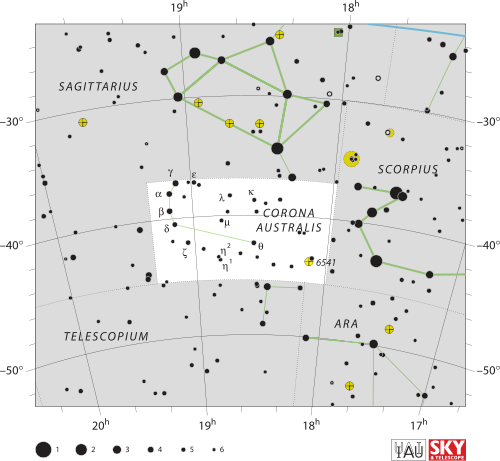
\includegraphics[scale=0.4]{CRA.png}
\caption{Corona Australis [5]\label{la}}
\end{figure}


\section{Observaciones}

Todas las observaciones se han llevado acabo en el observatorio astronomico de la 
Universidad de los Andes. A continuaci\'on se describen la instrumentacion utlizada
as\'i como los protocolos de observaci\'on utilizados.

El montaje experimental que se utilizo se muestra en la Fig. \ref{montaje} en el cual se ve el acople
de las fibras \'opticas al telescopio, por medio de estas fibras las luz es llevada hasta
el espectr\'ografo.

\subsection{Instrumentaci\'on}

\subsubsection{Telescopio}

Se utiliz\'o un telescopio marca Meade LX200 Schimdt-Cassegrain Fig.\ref{la} de $40 cm$ de apertura y una
distancia focal de $4m$.

\begin{figure}señalan
\centering
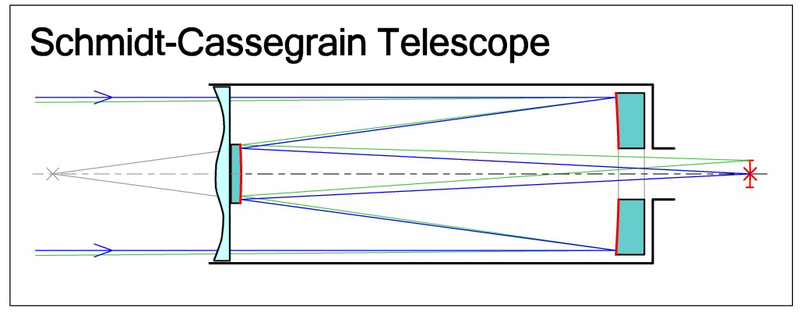
\includegraphics[scale=0.4]{SCT2.jpg}
\caption{Camino de luz en un telescopio Schmidt-Cassegrain [6] \label{la}}
\end{figure}


\subsubsection{Espectrografo}

El espectr\'rografo que se utilizo (Espartaco) Fig.\ref{espectrografo} es un espectrografo de alta resolucion en el cual la luz del telescopio llega por medio de una fibra \'optica, luego esta luz es descompuesta por una rendija de difracci\'on y finalmente la radiaci\'on es recolectada en una CCD.


\begin{figure}
\centering
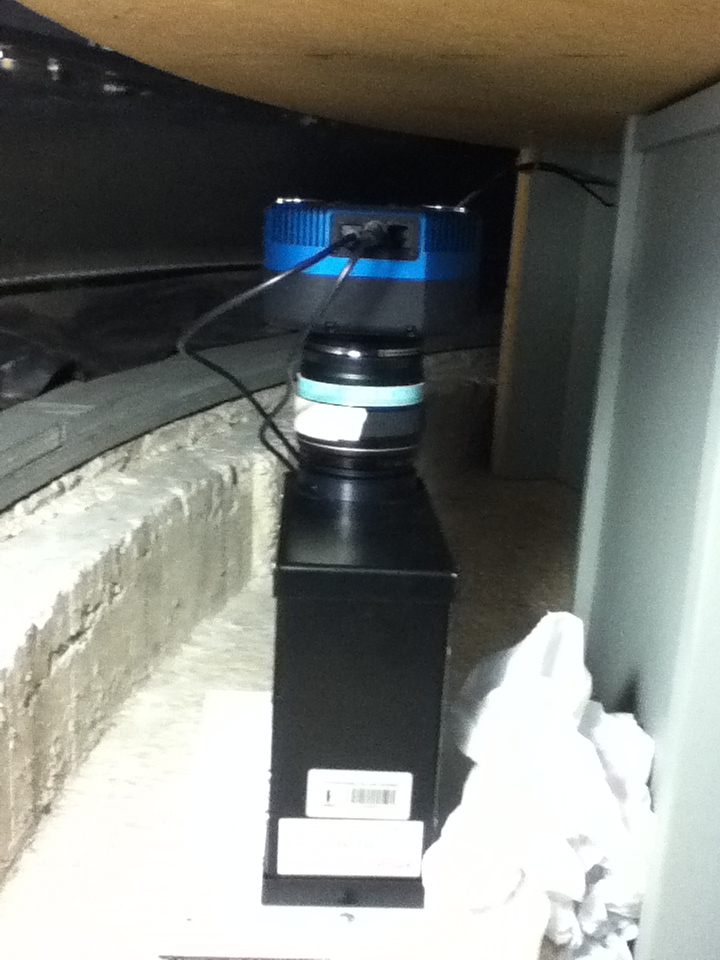
\includegraphics[scale=0.2]{espectroscopio.jpg}
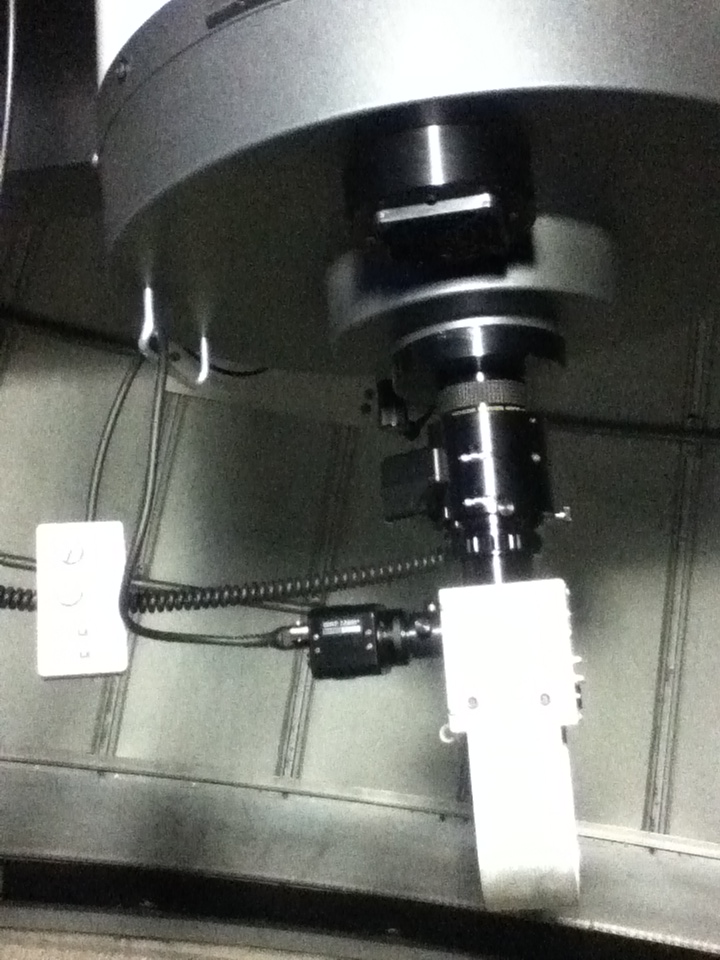
\includegraphics[scale=0.2]{montaje.jpg}
\caption{Espectrografo (Izquierda), Montaje experimental (Derecha)\label{espectrografo}}
\end{figure}



\subsubsection{Software}

La reducci\'on de datos se llevo acabo con el software ISIS [4]
el cual usa como referencia los espectros de las lamparas de calibracion (de torio y tungsteno)
para obtener los perfiles de los espectros tomados de las estrellas.

\subsection{Protocolo de Observacion}

Todas las observaciones se han llevado acabo en el observatorio de astronomico
de la universidad de los andes. Los datos ac\'a presentados se tomaron las noches
del 10, 13 y 16 de septiembre de 2013. En un intervalo de tiempo aproximadamente 
desde las 5pm hasta las 10 pm. 

El protocolo de observacion que se sigio fue el siguiente:

\begin{itemize}
\item Preparar el montaje, conectar el espectroscopio al telescopio haciendo de las 
fibras opticas.
\item Tomar espectros de las lamparas de calibraci\'on 
\item Posicionar la fibra optica en el foco del telescopio
\item Encontrar la estrella binaria $\varepsilon CRA$ y enfocarla en la fibra optica
\item Tomar los espectros, entre 5 y 15 min cada uno.
\end{itemize}

\section{Discusion y resultados}

De los espectros observados para $\varepsilon CRA$ ninguno presenta 
lineas dobles [poner referencia de github con las imagenes], sin estas lineas dibles no es posible obtener informacion 
relevante sobra la orbita de la binaria. Por lo tanto con estos espectros
calcularemos la velocidad radial del sistema, y se usaran los espectros
de Spica (otra binaria) previamnete tomados en el mismo telescopio con el fin de hacer el analisis de la orbita de Spica.

\subsection{Velocidad radial de $\varepsilon CRA$}

En la tabla\ref{spectra} se encuentra un resumen de los espectros tenidos en cuenta para encontrar la velocidad radial.\\

\begin{table}
\begin{center}
\begin{tabular}{|c| c |c|}
\hline
Nombre & Fecha & Hora\\
\hline
$Sept10EpscraA$ & Septiembre 10 & $14.254$\\
\hline
$Sept10EpscraB$ & Septiembre 10 & $14.254$\\
\hline
$Sept10EpscraC$ & Septiembre 10 & $14.254$\\
\hline
$Sept13EpscraA$ & Septiembre 13 & $13.996$\\
\hline
$Sept13EpscraB$ & Septiembre 13 & $14.039$\\
\hline
$Sept13EpscraC$ & Septiembre 13 & $14.062$\\
\hline
$Oct15A$ & octubre 15 & $16.007$\\
\hline
$Oct15B$ & octubre 15 & $16.016$\\
\hline
$Oct15C$ & octubre 15 & $16.032$\\
\hline
$Oct15D$ & octubre 15 & $16.045$\\
\hline
$Oct15E$& octubre 15 & $16.057$\\
\hline
$Oct15F$ & octubre 15 & $16.070$\\
\hline
\end{tabular}
\caption{Espectros utilizados\label{spectra}}
\end{center}
\end{table}


Para hallar la velocidad radial primero identificamos las lineas que tengan mejor perfil (en su mayoria son las de FeI y FeII) es decir que no sean tan anchas y sobresalgan del continuo.
En la Fig.\ref{espectra} se muestra las lineas que se escogieron para el $Oct15F$. Para hallar las longitud de onda observada
se escogia respecto el centro de la linea i.e el punto en el cual la intensidad corresponde al FWHM. \\

Las barras de error corresponden al error a la hora de encontrar la longitud observada, as\'i el error en logntiud de onda aparentemente no sea tan significativo $\sim 0.1 \AA$ este error 
en velocidad si es considerable $\sim 7 kms^{-1}$. \\ 

Tambien hay presencia de lineas mezcladas, es decir en una aparante linea pueden haber dos o m\'as lineas de distintos 
elementos. Esto hace que el centro de la linea se vea modificiado lo cual cambiaria la longitud de onda observada, 
un m\'etodo para evitar esto es ajustar funciones Gaussianas a cada una de las lineas y as\'i separarlas y saber con exactitud el centro de la linea.\\

\begin{figure}
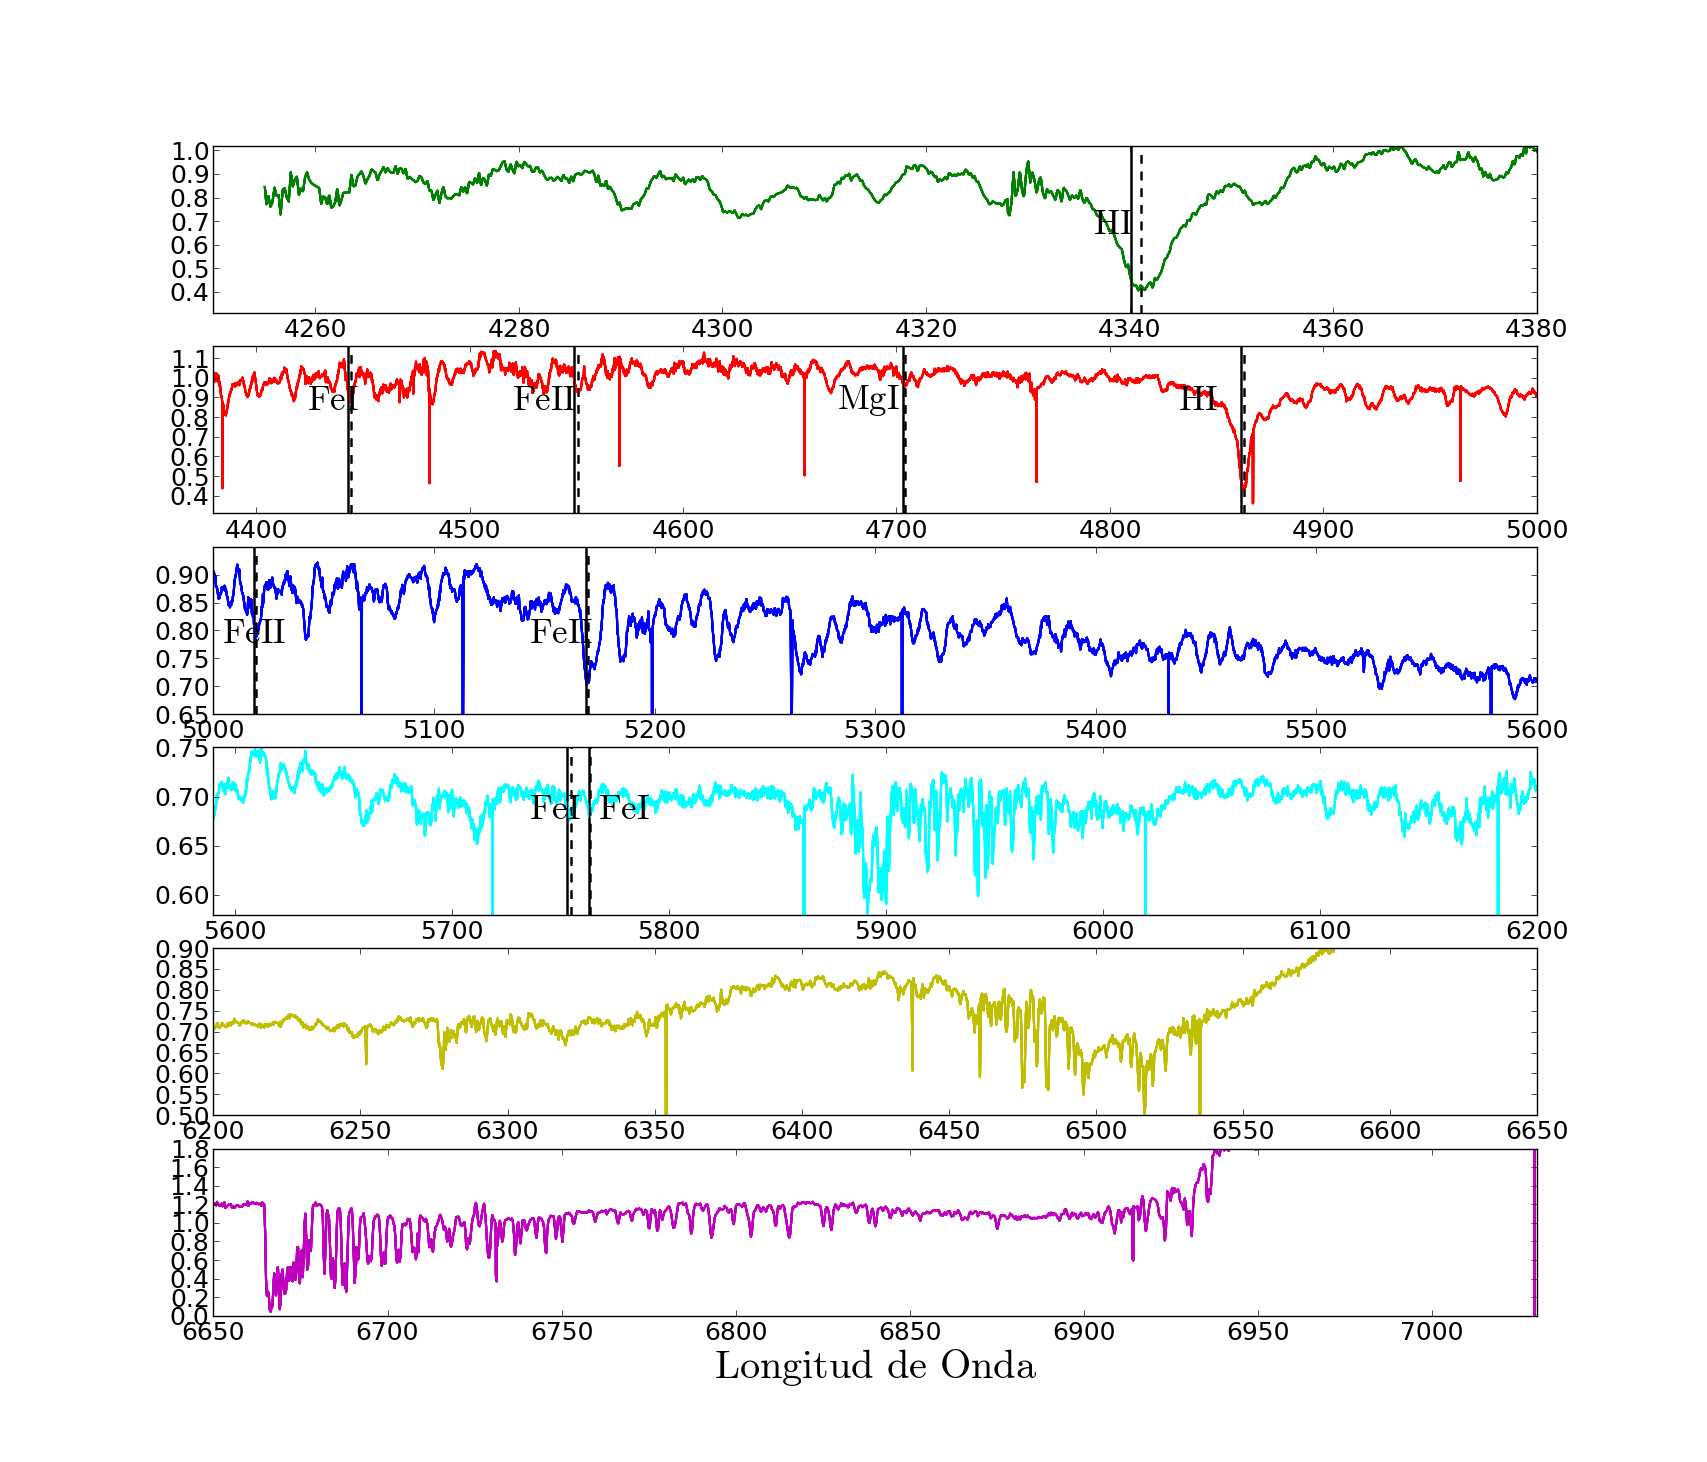
\includegraphics[scale=0.3]{spectra.png}
\caption{Espectros de $\varepsilon CRA$ tomados el 15/oct/2013
las lineas punteadas corresponden a la longitud de onda observada, las 
lineas solidas corresponden a la longitud de onda emitida esta ulitma se tomo de [XXX]\label{espectra}}
\end{figure}

Haciendo uso de \eqref{v} se encontro la velocidad para cada linea Fig\ref{vradial} cuyo valor promedio fue de $55.285 \pm 6.59 Km s^{-1}$ el error porcentual respecto al valor reportado por \ref{brimel} $57.9 \pm 1.2 Kms^{-1}$ fue de $4.51\%$. \\

\begin{figure}
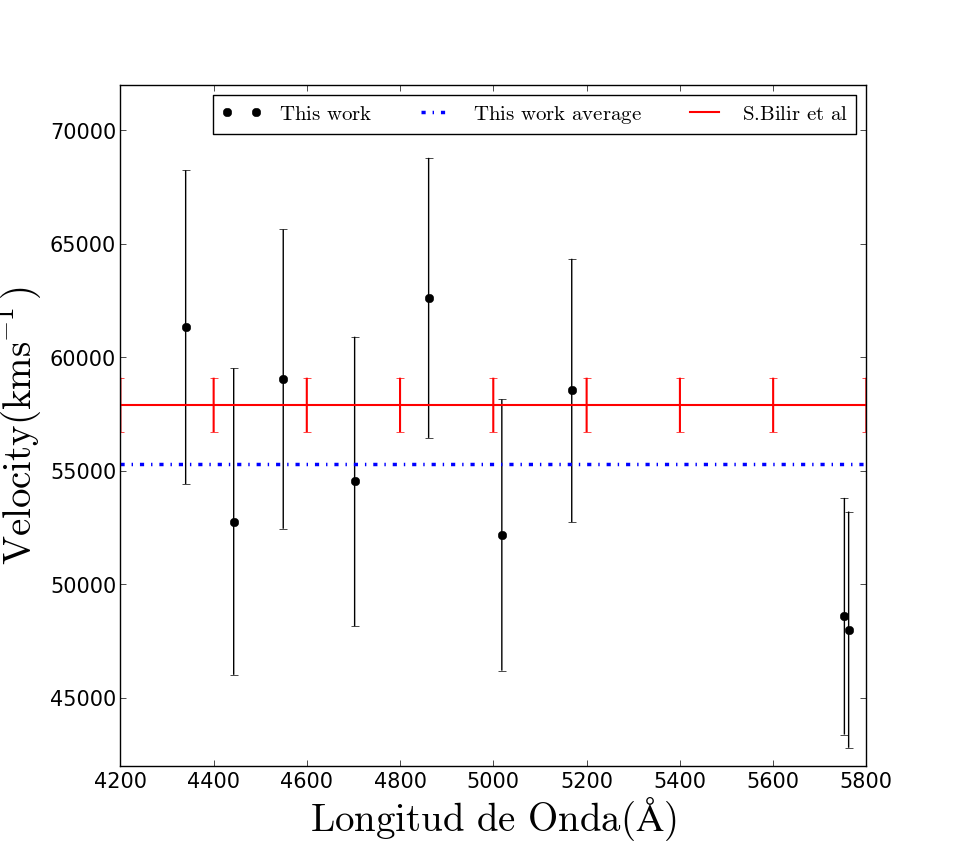
\includegraphics[scale=0.5]{radialvelocity.png}
\caption{Velocidad Radial de cada una de las lin\'eas en funci\'on de la longitud de onda. La linea roja representa el valor reportado por S.Bilir et al (2005), la azul punteada el valor promedio encontrado con [nombre dle espectro] de $v=55.285 \pm 6.59 Kms^{-1}$\label{vradial}}
\end{figure}

Con el fin de buscar alg\'un indicio del la orbita en el espectro de $\varepsilon CRA$ buscamos efectos tales como 
el ensanchamiento de la linea o alguna relacion velocidad radial/fase. Donde la fase representa el moemnto en el cual el 
sistema binario esta.\\

Para esto se utilizaron todos los espectros tomados en Octubre 15. En la Fig.\ref{AllSpectra} se muestra como el centro de la linea se ve ligeremante afectado por la diferencia de tiempo en la que son tomados los espectros.\\

\begin{figure}
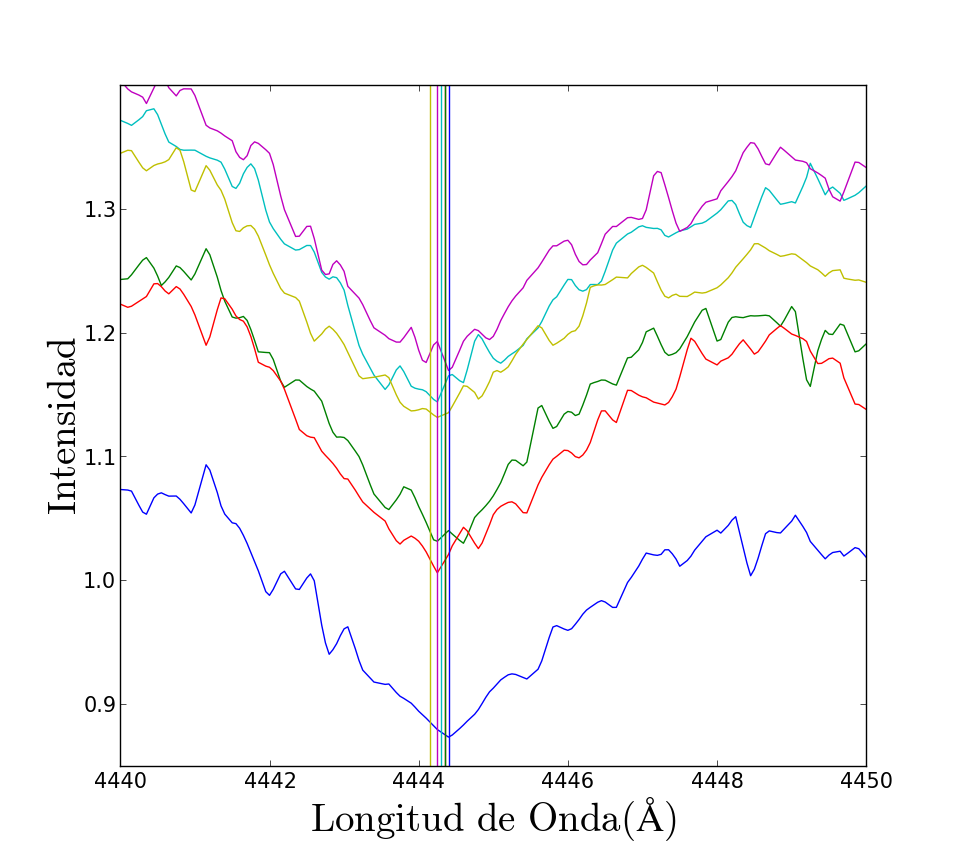
\includegraphics[scale=0.5]{epscraEspectra.png}
\caption{Velocidad radial para todos los espectros de Octubre 15. \label{AllSpectra}}
\end{figure}

\begin{figure}
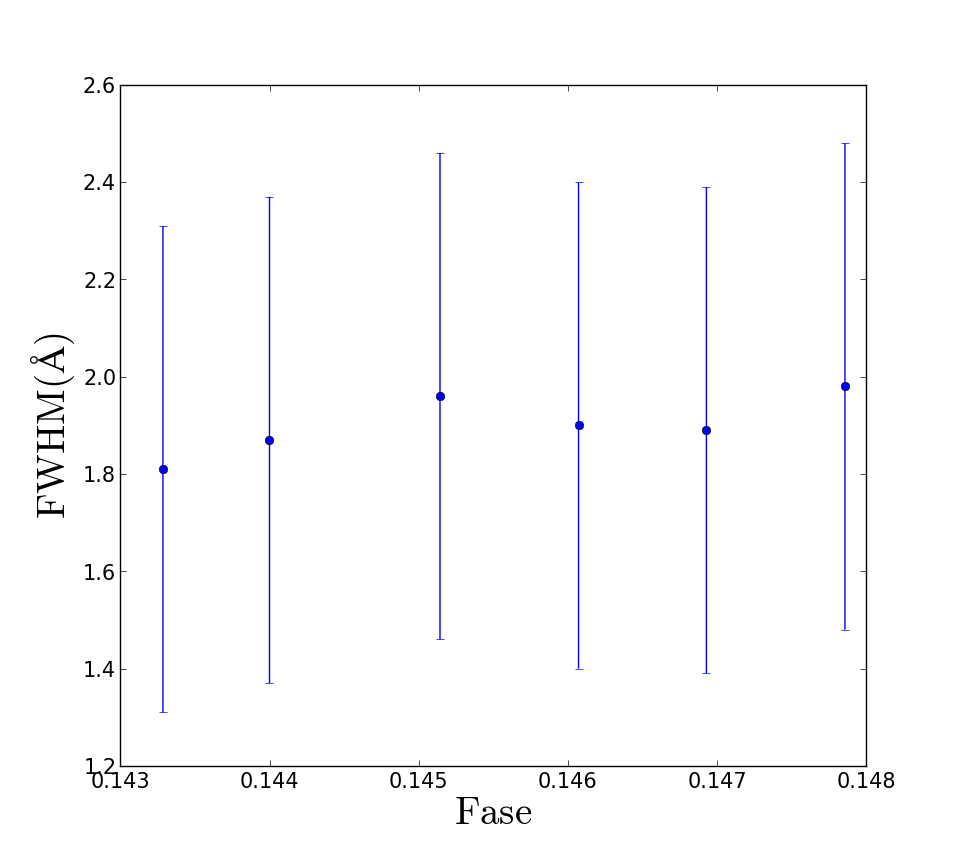
\includegraphics[scale=0.5]{anchovsfase.png}
\caption{Velocidad radial para todos los espectros de Octubre 15. \label{FWHM}}
\end{figure}

\begin{figure}
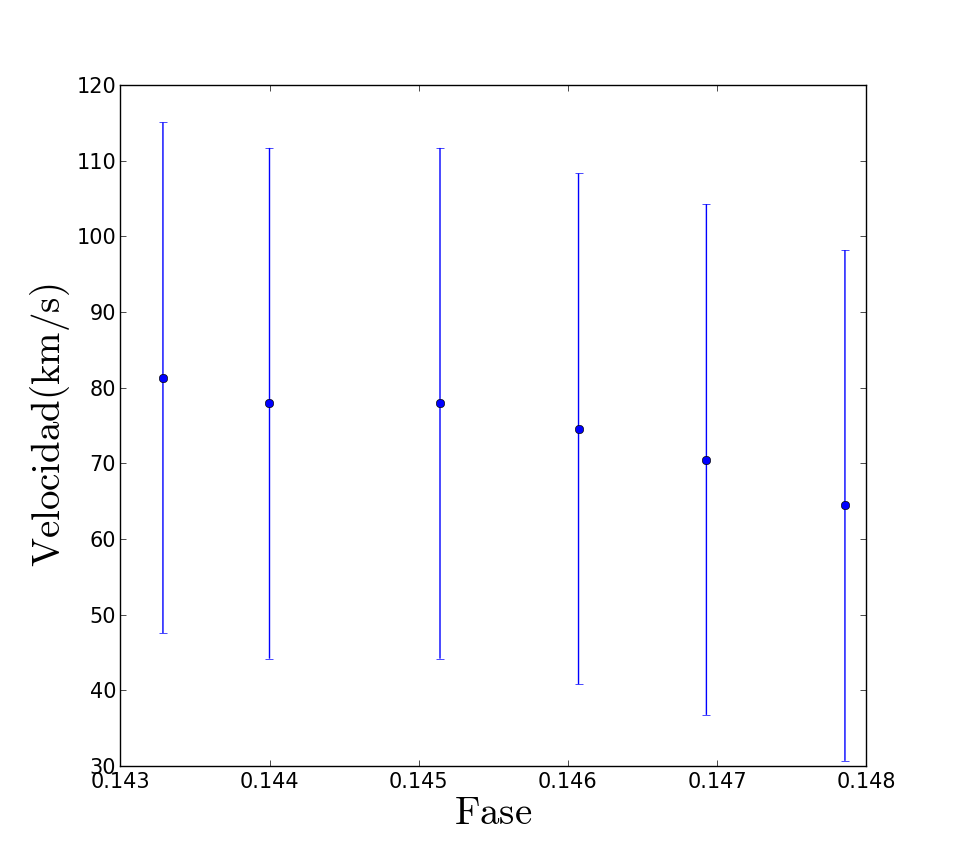
\includegraphics[scale=0.5]{velocidadvsfase.png}
\caption{Velocidad radial para todos los espectros de Octubre 15. \label{vvsfase}}
\end{figure}


Todos los datos tomados estan disponible en:

$ https://github.com/jngaravitoc/EpsCra/tree/master/data.$

El desarrollo para encontrar las velocidades radiales esta 
disponible en:

$http://nbviewer.ipython.org/urls/raw.github.com/jngaravitoc/EpsCra/master/Spectra_analysis.ipynb
$
\subsection{Periodo Orbital de Spica}


\section{Conclusiones}

\section{Agradecimientos}

JNGC agradece a BO por su infantable y tiempo
asi como tambien a Juan Camilo Buitrago Astr\'onomo encargo
del observatorio  

\section{Referencias}

1. $http://ned.ipac.caltech.edu$  \\
2. Karttunen, Fundamental astronomy 5th edition.\\
3. Alan H. Batten, J. Murray Fletcher and D. G. MacCarthy, http://ad.usno.navy.mil/wds/dsl/SB8/sb8.html\\
4. $http://www.astrosurf.com/buil/isis/isis_en.htm$\\
5. http://www.iau.org/static/public/constellations/gif/CRA.gif \\
6. http://en.wikipedia.org/wiki/File:Schmidt-Cassegrain-Telescope.png \\
7. http://simbad.u-strasbg.fr/simbad/sim-id?Ident=%402353328&Name=V*%20eps%20CrA&submit=submit

\end{document}
